\section{Analysis strategy}\label{sec:AnalysisStrategy}

\subsection{Introduction}
The analysis strategy for the high mass search with 2016 data in the
$\mathrm{W^+W^-}\to2\ell2\nu$ decay channel  is similar to the previous high
mass analysis with 2015 data~\cite{CMS-PAS-HIG-16-023}, but has several improvements. \\
In the opposite-flavour $\mathrm{W^+W^-}\to e^{\pm} \mu^{\mp} 2\nu$ final
state four different jets-categories are defined (they were three in
~\cite{CMS-PAS-HIG-16-023}): 0-jet, 1-jet, 2-jet-non VBF and VBF. The 2 jet
non-VBF category is new with respect to ~\cite{CMS-PAS-HIG-16-023}.
A same-flavour (SF) $\mathrm{W^+W^-}\to e^+ e^- 2\nu$ and $\mathrm{W^+W^-}\to
\mu^+ \mu^- 2\nu$ category, has been added in the VBF phase space. Indeed, the VBF
selection cuts are sufficiently tight to reduce the otherwise overwhelming
Z+jets background to a manageable level.

Whenever we count jets in this analysis we always refer to AK4 jets with $\pt>30$\GeV.

Events are requested to pass single or double lepton triggers. Leptons should have a mini-
mum $p_T$ of 10 (13) GeV for the muon (electron) candidate. One of the two leptons should also
have a $p_T$ greater than 25 GeV and two leptons are requested to be well identified and isolated,
to reject non-prompt leptons and leptons coming from QCD sources. These selections are in
common to all phase spaces, and are detailed in~\cite{AN-17-082}.


The main production mode for the Higgs boson production over the all mass spectrum is the gluon-gluon fusion process (ggH). At a center-of-mass energy of 13\TeV the ggH cross section for a Higgs boson mass ($m_\mathrm{H}$) of 125\GeV is 43.92\,pb~\cite{temphiggsxsecs}, that is almost one order of magnitude larger than the second process  in terms of cross section at that mass, VBF, with 3.748\,pb~\cite{temphiggsxsecs}. The ggH cross section decreases with $m_\mathrm{H}$ but the VBF/ggH cross section ratio increases with the mass, making the VBF production mechanism more and more important as $m_\mathrm{H}$ approaches to high values.\\
The signal samples are interpreted in terms of the EWK singlet model described
in Sec~\ref{sec:signalModel} below. The Higgs boson width and lineshape is reweighted at generator level according to the parameters defined in the model.
The interference effects between the ggH signal, the ggWW background and SM
Higgs boson, that are expected to slightly change the lineshape of the signal
distribution, have been fully taken into account, as detailed in
Sec.~\ref{sec:interference}. A similar treatment is also applied for the
intereference between the VBF high mass signal, the VBF SM Higgs and the quark
initiated WW+2 quarks backgrround. The interference between the $\mathrm{W^+W^-}\to2\ell2\nu$ and $\mathrm{ZZ}\to2\ell2\nu$ is negligible due to the different phase space characteristic of these processes. 

\subsection{Discriminating variable}
The analysis presented in this note is a shape analysis, meaning that after
applying selection cuts detailed in Secs~.\ref{sec:OF} and \ref{sec:SF} below,
we do not simply count events, but rather we fit a data histogram of a
discriminating variable with the sum of signal and background templates, and
extract the signal yield from the fit.
The variable with the best discriminating value would be the invariant mass of
the four lepton, which is not possible to reconstruct in the \WW channel due
to neutrinos.
%The branching fraction from Higgs to a \WW pair is the largest for mass values above 200\GeV~\cite{Heinemeyer:2013tqa}, and the $\mathrm{W^+W^-}\to2\ell2\nu$ decay channel is the second in terms of branching ratio, surpassed only by the semi-leptonic decay mode. 
%In addition  the leptonic decay chosen boasts a very clear experimental signature,  and though there are several backgrounds affecting the final state,  
%there are some kinematic variables that can be used to separate the signal, leading to a good and clearn signal sensitivity.

In the SM Higgs analysis (HIG-16-042),  a shape analysis based on two-dimensional templates of $m_{\ell \ell}$ versus $m_T^H$ in each of the categories is performed, where  the transverse mass  $m_T^H$ variable is defined as  
\begin{equation}
 m_T^H = \sqrt{2p_{\rm T}^{\ell\ell}\MET(1-\mathrm{cos}\Delta\phi(\ell\ell, \ptvecmiss))}
\end{equation}
where $\Delta\phi(\ell\ell, \ptvecmiss)$ is the azimuthal angle between the dilepton momentum and \ptvecmiss.\\
However  $m_T^H$ (and also $m_{\ell \ell}$) is not very sensitive to the
signal mass hypothesis, so a \textit{new} variable $m_T^I$ defined as the visible mass,
\begin{equation}
 m_T^I = \sqrt{ (p_\mathrm{\ell\ell} + \MET)^2 - (\vec{p}_\mathrm{\ell\ell} + \ptvecmiss)^2 }
\end{equation}
has been introduced in 2015 analysis to discriminate better the signals generate at different masses.
The distribution of the variables defined above are shown in
Fig.~\ref{fig:mt_nocuts}, where the better power of $m_T^I$ in discriminating
different mass hypotheses over other variable is visible.

\begin{figure}[htbp]
\centering
\subfigure[True generated mass]{
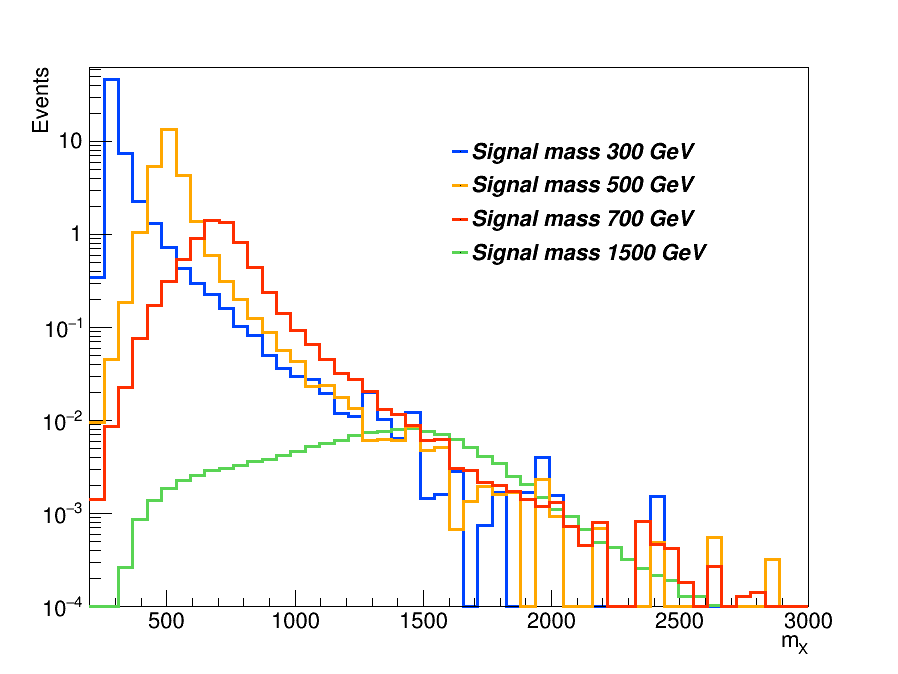
\includegraphics[width=0.45\textwidth]{../AN/Figs/Distribution_higgsLHEmass_cuts_nocuts.png}
}
\subfigure[$m_T^H$]{
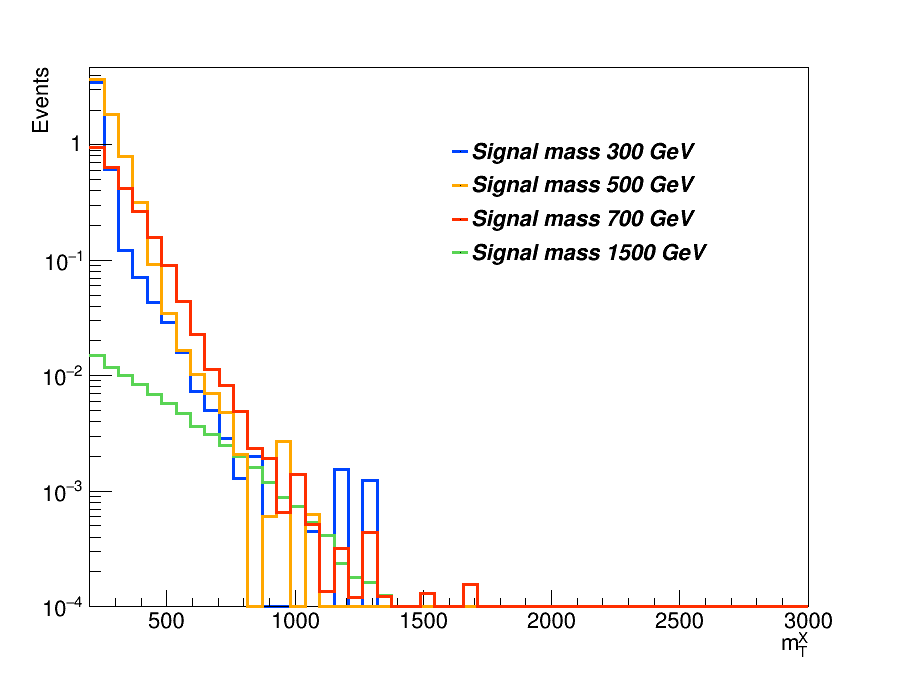
\includegraphics[width=0.45\textwidth]{../AN/Figs/Distribution_mth_cuts_nocuts.png}
}
\\
\subfigure[$m_{\ell \ell}$]{
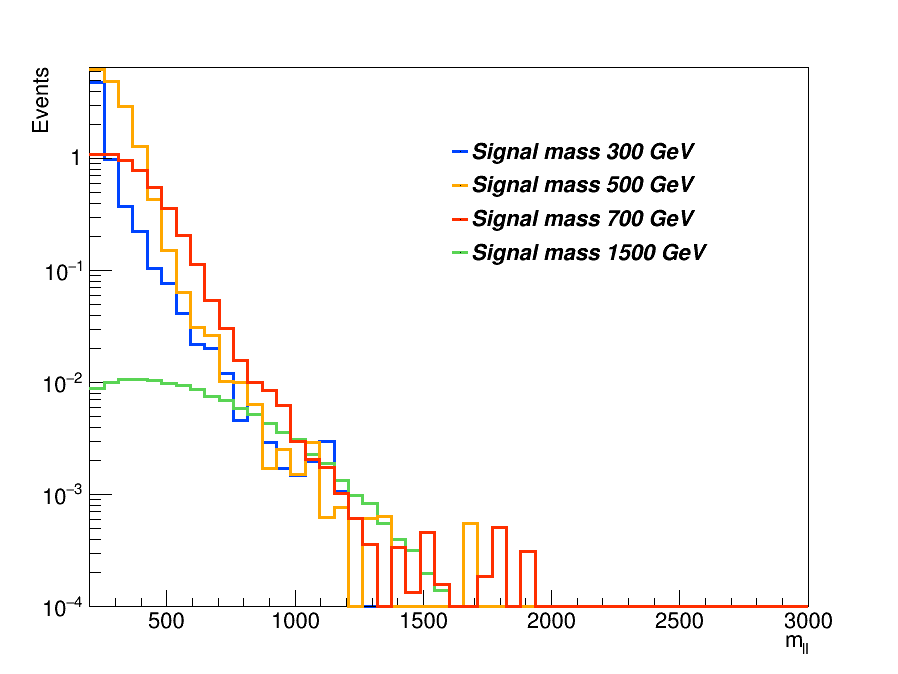
\includegraphics[width=0.45\textwidth]{../AN/Figs/Distribution_mll_cuts_nocuts.png}
}
\subfigure[$m_T^I$]{
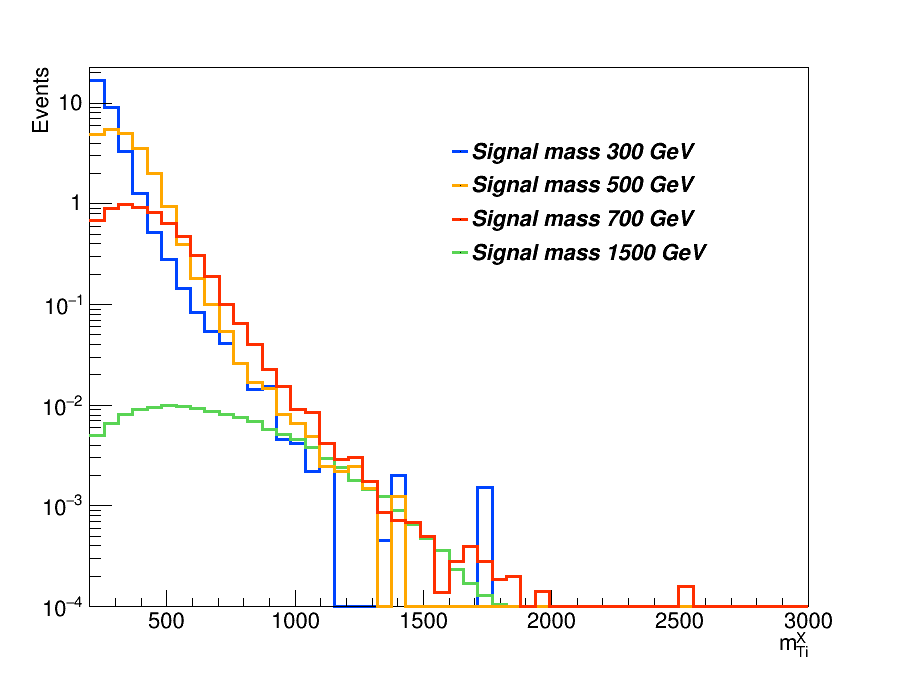
\includegraphics[width=0.45\textwidth]{../AN/Figs/Distribution_mTi_cuts_nocuts.png}
}
\caption{
    Distributions of the generated mass, $m_T^H$, $m_{\ell \ell}$ and  $m_T^I$
    variables for different Higgs mass hypothesis, without
    any selection. The same distribution after the OF selection are shown in Appendix \ref{sec:AppA}.}
    \label{fig:mt_nocuts}
\end{figure}


